\documentclass[
a4paper,     %% defines the paper size: a4paper (default), a5paper, letterpaper, ...
% landscape,   %% sets the orientation to landscape
% twoside,     %% changes to a two-page-layout (alternatively: oneside)
% twocolumn,   %% changes to a two-column-layout
% headsepline, %% add a horizontal line below the column title
% footsepline, %% add a horizontal line above the page footer
% titlepage,   %% only the titlepage (using titlepage-environment) appears on the first page (alternatively: notitlepage)
% parskip,     %% insert an empty line between two paragraphs (alternatively: halfparskip, ...)
% leqno,       %% equation numbers left (instead of right)
% fleqn,       %% equation left-justified (instead of centered)
% tablecaptionabove, %% captions of tables are above the tables (alternatively: tablecaptionbelow)
% draft,       %% produce only a draft version (mark lines that need manual edition and don't show graphics)
% 10pt         %% set default font size to 10 point
% 11pt         %% set default font size to 11 point
11pt         %% set default font size to 12 point
]{scrartcl}  %% article, see KOMA documentation (scrguide.dvi)


\usepackage[pdftex]{graphicx}
\usepackage{caption}
\usepackage{subcaption}
\usepackage{tikz}
%\usepackage{pgfplots}

\usetikzlibrary{spy,calc}

\newif\ifblackandwhitecycle
\gdef\patternnumber{0}

\pgfkeys{/tikz/.cd,
    zoombox paths/.style={
        draw=orange,
        very thick
    },
    black and white/.is choice,
    black and white/.default=static,
    black and white/static/.style={ 
        draw=white,   
        zoombox paths/.append style={
            draw=white,
            postaction={
                draw=black,
                loosely dashed
            }
        }
    },
    black and white/static/.code={
        \gdef\patternnumber{1}
    },
    black and white/cycle/.code={
        \blackandwhitecycletrue
        \gdef\patternnumber{1}
    },
    black and white pattern/.is choice,
    black and white pattern/0/.style={},
    black and white pattern/1/.style={    
            draw=white,
            postaction={
                draw=black,
                dash pattern=on 2pt off 2pt
            }
    },
    black and white pattern/2/.style={    
            draw=white,
            postaction={
                draw=black,
                dash pattern=on 4pt off 4pt
            }
    },
    black and white pattern/3/.style={    
            draw=white,
            postaction={
                draw=black,
                dash pattern=on 4pt off 4pt on 1pt off 4pt
            }
    },
    black and white pattern/4/.style={    
            draw=white,
            postaction={
                draw=black,
                dash pattern=on 4pt off 2pt on 2 pt off 2pt on 2 pt off 2pt
            }
    },
    zoomboxarray inner gap/.initial=5pt,
    zoomboxarray columns/.initial=2,
    zoomboxarray rows/.initial=2,
    subfigurename/.initial={},
    figurename/.initial={zoombox},
    zoomboxarray/.style={
        execute at begin picture={
            \begin{scope}[
                spy using outlines={%
                    zoombox paths,
                    width=\imagewidth / \pgfkeysvalueof{/tikz/zoomboxarray columns} - (\pgfkeysvalueof{/tikz/zoomboxarray columns} - 1) / \pgfkeysvalueof{/tikz/zoomboxarray columns} * \pgfkeysvalueof{/tikz/zoomboxarray inner gap} -\pgflinewidth,
                    height=\imageheight / \pgfkeysvalueof{/tikz/zoomboxarray rows} - (\pgfkeysvalueof{/tikz/zoomboxarray rows} - 1) / \pgfkeysvalueof{/tikz/zoomboxarray rows} * \pgfkeysvalueof{/tikz/zoomboxarray inner gap}-\pgflinewidth,
                    magnification=3,
                    every spy on node/.style={
                        zoombox paths
                    },
                    every spy in node/.style={
                        zoombox paths
                    }
                }
            ]
        },
        execute at end picture={
            \end{scope}
            \node at (image.north) [anchor=north,inner sep=0pt] {\subcaptionbox{\label{\pgfkeysvalueof{/tikz/figurename}-image}}{\phantomimage}};
            \node at (zoomboxes container.north) [anchor=north,inner sep=0pt] {\subcaptionbox{\label{\pgfkeysvalueof{/tikz/figurename}-zoom}}{\phantomimage}};
     \gdef\patternnumber{0}
        },
        spymargin/.initial=0.5em,
        zoomboxes xshift/.initial=1,
        zoomboxes right/.code=\pgfkeys{/tikz/zoomboxes xshift=1},
        zoomboxes left/.code=\pgfkeys{/tikz/zoomboxes xshift=-1},
        zoomboxes yshift/.initial=0,
        zoomboxes above/.code={
            \pgfkeys{/tikz/zoomboxes yshift=1},
            \pgfkeys{/tikz/zoomboxes xshift=0}
        },
        zoomboxes below/.code={
            \pgfkeys{/tikz/zoomboxes yshift=-1},
            \pgfkeys{/tikz/zoomboxes xshift=0}
        },
        caption margin/.initial=4ex,
    },
    adjust caption spacing/.code={},
    image container/.style={
        inner sep=0pt,
        at=(image.north),
        anchor=north,
        adjust caption spacing
    },
    zoomboxes container/.style={
        inner sep=0pt,
        at=(image.north),
        anchor=north,
        name=zoomboxes container,
        xshift=\pgfkeysvalueof{/tikz/zoomboxes xshift}*(\imagewidth+\pgfkeysvalueof{/tikz/spymargin}),
        yshift=\pgfkeysvalueof{/tikz/zoomboxes yshift}*(\imageheight+\pgfkeysvalueof{/tikz/spymargin}+\pgfkeysvalueof{/tikz/caption margin}),
        adjust caption spacing
    },
    calculate dimensions/.code={
        \pgfpointdiff{\pgfpointanchor{image}{south west} }{\pgfpointanchor{image}{north east} }
        \pgfgetlastxy{\imagewidth}{\imageheight}
        \global\let\imagewidth=\imagewidth
        \global\let\imageheight=\imageheight
        \gdef\columncount{1}
        \gdef\rowcount{1}
        \gdef\zoomboxcount{1}
    },
    image node/.style={
        inner sep=0pt,
        name=image,
        anchor=south west,
        append after command={
            [calculate dimensions]
            node [image container,subfigurename=\pgfkeysvalueof{/tikz/figurename}-image] {\phantomimage}
            node [zoomboxes container,subfigurename=\pgfkeysvalueof{/tikz/figurename}-zoom] {\phantomimage}
        }
    },
    color code/.style={
        zoombox paths/.append style={draw=#1}
    },
    connect zoomboxes/.style={
    spy connection path={\draw[draw=none,zoombox paths] (tikzspyonnode) -- (tikzspyinnode);}
    },
    help grid code/.code={
        \begin{scope}[
                x={(image.south east)},
                y={(image.north west)},
                font=\footnotesize,
                help lines,
                overlay
            ]
            \foreach \x in {0,1,...,9} { 
                \draw(\x/10,0) -- (\x/10,1);
                \node [anchor=north] at (\x/10,0) {0.\x};
            }
            \foreach \y in {0,1,...,9} {
                \draw(0,\y/10) -- (1,\y/10);                        \node [anchor=east] at (0,\y/10) {0.\y};
            }
        \end{scope}    
    },
    help grid/.style={
        append after command={
            [help grid code]
        }
    },
}

\newcommand\phantomimage{%
    \phantom{%
        \rule{\imagewidth}{\imageheight}%
    }%
}
\newcommand\zoombox[2][]{
    \begin{scope}[zoombox paths]
        \pgfmathsetmacro\xpos{
            (\columncount-1)*(\imagewidth / \pgfkeysvalueof{/tikz/zoomboxarray columns} + \pgfkeysvalueof{/tikz/zoomboxarray inner gap} / \pgfkeysvalueof{/tikz/zoomboxarray columns} ) + \pgflinewidth
        }
        \pgfmathsetmacro\ypos{
            (\rowcount-1)*( \imageheight / \pgfkeysvalueof{/tikz/zoomboxarray rows} + \pgfkeysvalueof{/tikz/zoomboxarray inner gap} / \pgfkeysvalueof{/tikz/zoomboxarray rows} ) + 0.5*\pgflinewidth
        }
        \edef\dospy{\noexpand\spy [
            #1,
            zoombox paths/.append style={
                black and white pattern=\patternnumber
            },
            every spy on node/.append style={#1},
            x=\imagewidth,
            y=\imageheight
        ] on (#2) in node [anchor=north west] at ($(zoomboxes container.north west)+(\xpos pt,-\ypos pt)$);}
        \dospy
        \pgfmathtruncatemacro\pgfmathresult{ifthenelse(\columncount==\pgfkeysvalueof{/tikz/zoomboxarray columns},\rowcount+1,\rowcount)}
        \global\let\rowcount=\pgfmathresult
        \pgfmathtruncatemacro\pgfmathresult{ifthenelse(\columncount==\pgfkeysvalueof{/tikz/zoomboxarray columns},1,\columncount+1)}
        \global\let\columncount=\pgfmathresult
        \ifblackandwhitecycle
            \pgfmathtruncatemacro{\newpatternnumber}{\patternnumber+1}
            \global\edef\patternnumber{\newpatternnumber}
        \fi
    \end{scope}
}
 %%% File-Information {{{
%%% Filename: template_bericht.tex
%%% Purpose: lab report, technical report, project report
%%% Time-stamp: <2004-06-30 18:19:32 mp>
%%% Authors: The LaTeX@TUG-Team [http://latex.tugraz.at/]:
%%%          Karl Voit (vk), Michael Prokop (mp), Stefan Sollerer (ss)
%%% History:
%%%   20050914 (ss) correction of "backref=true" to "backref" due to hyperref documentation
%%%   20040630 (mp) added comments to foldmethod at end of file
%%%   20040625 (vk,ss) initial version
%%%
%%% Notes:
%%%
%%%
%%%
%%% }}}


%%%%%%%%%%%%%%%%%%%%%%%%%%%%%%%%%%%%%%%%%%%%%%%%%%%%%%%%%%%%%%%%%%%%%%%%%%%%%%%%
%%%
%%% packages
%%%


\usepackage[a4paper]{geometry}
\geometry{tmargin=1in,bmargin=1.25in,lmargin=2.5cm,rmargin=2cm}

\usepackage{microtype}

%%%
%%% encoding and language set
%%%

%%% ngerman: language set to new-german
\usepackage[english]{babel} 
\usepackage{tocloft}
\usepackage{subcaption}
\usepackage{listings}
\usepackage{color} %red, green, blue, yellow, cyan, magenta, black, white
\usepackage{courier}
\usepackage{float}

\usepackage{siunitx}

%%% babel: language set (can cause some conflicts with package ngerman)
%%%        use it only for multi-language documents or non-german ones
%\usepackage[ngerman]{babel}

%%% inputenc: coding of german special characters
\usepackage[latin1]{inputenc}

%%% fontenc, ae, aecompl: coding of characters in PDF documents
\usepackage[T1]{fontenc}
\usepackage{ae,aecompl}

%%%
%%% technical packages
%%%

%%% amsmath, amssymb, amstext: support for mathematics
%\usepackage{amsmath,amssymb,amstext}

\usepackage{bm}

%%% psfrag: replace PostScript fonts
\usepackage{psfrag}

%%% listings: include programming code
%\usepackage{listings}

%%% units: technical units
%\usepackage{units}

%%%
%%% layout
%%%

%%% scrpage2: KOMA heading and footer
%%% Note: if you don't use this package, please remove 
%%%       \pagestyle{scrheadings} and corresponding settings
%%%       below too.
\usepackage[automark]{scrpage2}


%%%
%%% PDF
%%%

\usepackage{ifpdf}

%%% Should be LAST usepackage-call!
%%% For docu on that, see reference on package ``hyperref''
\ifpdf%   (definitions for using pdflatex instead of latex)

  %%% graphicx: support for graphics
  \usepackage[pdftex]{graphicx}

  \pdfcompresslevel=9

  %%% hyperref (hyperlinks in PDF): for more options or more detailed
  %%%          explanations, see the documentation of the hyperref-package
  \usepackage[%
    %%% general options
    %pdftex=true,      %% sets up hyperref for use with the pdftex program
    %plainpages=false, %% set it to false, if pdflatex complains: ``destination with same identifier already exists''
    %
    %%% extension options
    backref,      %% adds a backlink text to the end of each item in the bibliography
    pagebackref=false, %% if true, creates backward references as a list of page numbers in the bibliography
    colorlinks=false,   %% turn on colored links (true is better for on-screen reading, false is better for printout versions)
    %
    %%% PDF-specific display options
    bookmarks=true,          %% if true, generate PDF bookmarks (requires two passes of pdflatex)
    bookmarksopen=false,     %% if true, show all PDF bookmarks expanded
    bookmarksnumbered=false, %% if true, add the section numbers to the bookmarks
    %pdfstartpage={1},        %% determines, on which page the PDF file is opened
    pdfpagemode=UseNone         %% None, UseOutlines (=show bookmarks), UseThumbs (show thumbnails), FullScreen
  ]{hyperref}


  %%% provide all graphics (also) in this format, so you don't have
  %%% to add the file extensions to the \includegraphics-command
  %%% and/or you don't have to distinguish between generating
  %%% dvi/ps (through latex) and pdf (through pdflatex)
  \DeclareGraphicsExtensions{.pdf}

\else %else   (definitions for using latex instead of pdflatex)

  \usepackage[dvips]{graphicx}

  \DeclareGraphicsExtensions{.eps}

  \usepackage[%
    dvips,           %% sets up hyperref for use with the dvips driver
    colorlinks=false %% better for printout version; almost every hyperref-extension is eliminated by using dvips
  ]{hyperref}

\fi


\usepackage[noabbrev]{cleveref}

%%% sets the PDF-Information options
%%% (see fields in Acrobat Reader: ``File -> Document properties -> Summary'')
%%% Note: this method is better than as options of the hyperref-package (options are expanded correctly)
\hypersetup{
  pdftitle={Image Based Measurement Laboratory}, %%
  pdfauthor={Filzmaier Josef, Michael Sieberer}, %%
  pdfsubject={Image Stitching, Auto-Focus, Sensor Dynamics, Perspective invariants}, %%
  pdfcreator={Accomplished with LaTeX2e and pdfLaTeX with hyperref-package.}, %% 
  pdfproducer={}, %%
  pdfkeywords={}, %%
  pdfnewwindow=true,      % links in new PDF window
  colorlinks=true,       % false: boxed links; true: colored links
  linkcolor=black,          % color of internal links (change box color with linkbordercolor)
  citecolor=black,        % color of links to bibliography
  filecolor=magenta,      % color of file links
  urlcolor=cyan           % color of external links
}


%%%%%%%%%%%%%%%%%%%%%%%%%%%%%%%%%%%%%%%%%%%%%%%%%%%%%%%%%%%%%%%%%%%%%%%%%%%%%%%%
%%%
%%% user defined commands
%%%

%%% \mygraphics{}{}{}
%% usage:   \mygraphics{width}{filename_without_extension}{caption}
%% example: \mygraphics{0.7\textwidth}{rolling_grandma}{This is my grandmother on inlinescates}
%% requires: package graphicx
%% provides: including centered pictures/graphics with a boldfaced caption below
%% 
\newcommand{\mygraphics}[3]{
  \begin{center}
    \includegraphics[width=#1, keepaspectratio=true]{#2} \\
    \textbf{#3}
  \end{center}
}

%%%%%%%%%%%%%%%%%%%%%%%%%%%%%%%%%%%%%%%%%%%%%%%%%%%%%%%%%%%%%%%%%%%%%%%%%%%%%%%%
%%%
%%% define the titlepage
%%%

 \subject{Image - Based Measurement Laboratory}   %% subject which appears above titlehead
 
 
%\titlehead{} %% special heading for the titlepage

%%% author(s)
\author{Filzmaier Josef (1030462) \and
Michael Sieberer (1531366)}

%%% date
\date{Graz, am \today{}}

% \publishers{}

% \thanks{} %% use it instead of footnotes (only on titlepage)

% \dedication{} %% generates a dedication-page after titlepage


%%% uncomment following lines, if you want to:
%%% reuse the maketitle-entries for hyperref-setup
%%\newcommand\org@maketitle{}
%%\let\org@maketitle\maketitle
%%\def\maketitle{%
%%  \hypersetup{
%%    pdftitle={\@title},
%%    pdfauthor={\@author}
%%    pdfsubject={\@subject}
%%  }%
%%  \org@maketitle
%%}


%%%%%%%%%%%%%%%%%%%%%%%%%%%%%%%%%%%%%%%%%%%%%%%%%%%%%%%%%%%%%%%%%%%%%%%%%%%%%%%%
%%%
%%% set heading and footer
%%%

%%% scrheadings default: 
%%%      footer - middle: page number
\pagestyle{scrheadings}

%%% user specific
%%% usage:
%%% \position[heading/footer for the titlepage]{heading/footer for the rest of the document}

%%% heading - left
% \ihead[]{}

%%% heading - center
% \chead[]{}

%%% heading - right
% \ohead[]{}

%%% footer - left
% \ifoot[]{}

%%% footer - center
% \cfoot[]{}

%%% footer - right
% \ofoot[]{}

\renewcommand*{\thesection}{Exercise~\arabic{section}:}
\renewcommand*{\thesubsection}{\arabic{section}.\arabic{subsection}}
\setlength{\cftsecnumwidth}{6.0em}
\setlength\parindent{0pt}
\definecolor{mygreen}{RGB}{28,172,0} % color values Red, Green, Blue
\definecolor{mylilas}{RGB}{170,55,241}
\lstset{language=Matlab,%
    basicstyle=\ttfamily\footnotesize,breaklines=true,
    breaklines=true,%
    morekeywords={matlab2tikz},
    keywordstyle=\color{blue},%
    morekeywords=[2]{1}, keywordstyle=[2]{\color{black}},
    identifierstyle=\color{black},%
    stringstyle=\color{mylilas},
    commentstyle=\color{mygreen},%
    showstringspaces=false,%without this there will be a symbol in the places where there is a space
    numbers=left,%
    numberstyle={\tiny \color{black}},% size of the numbers
    numbersep=9pt, % this defines how far the numbers are from the text
    emph=[1]{for,end,break},emphstyle=[1]\color{red}, %some words to emphasise
    captionpos=b,
    %emph=[2]{word1,word2}, emphstyle=[2]{style},    
}
\newcommand{\sidebysidepic}[6]{
\begin{figure}[ht!]%
\begin{subfigure}{.5\textwidth}%
  \centering%
  \includegraphics[width=.8\linewidth]{#1}%
  \caption{#2}%
\end{subfigure}%
\begin{subfigure}{.5\textwidth}%
  \centering%
  \includegraphics[width=.8\linewidth]{#3}%
  \caption{#4}%
\end{subfigure}%
\caption{#5}%
\label{#6}%
\end{figure}%
}
 

\usepackage{placeins}
\usepackage{tabu}
\usepackage{siunitx}
\usepackage{booktabs}
\usepackage{amsmath,amssymb}


%%% title
\title{Lab2 - Color}


%%%%%%%%%%%%%%%%%%%%%%%%%%%%%%%%%%%%%%%%%%%%%%%%%%%%%%%%%%%%%%%%%%%%%%%%%%%%%%%%
%%%
%%% begin document
%%%

\begin{document}

% \pagenumbering{roman} %% small roman page numbers

%%% include the title
% \thispagestyle{empty}  %% no header/footer (only) on this page
 \maketitle

%%% start a new page and display the table of contents
 \tableofcontents
 \newpage

\section{Image Acquisition}

\subsection{Problem statement}

Using a color camera perform the following tasks:

\begin{itemize}
 \item Acquire a set of images.
 \item Extract the raw image of the camera.
 \item Implement a MATLAB function which transforms the $N \times M \times 1$ raw image of the sensor into a $N \times M \times 3$ RGB image using a bilinear interpolation.
 \item Convert your images and discuss your results.
\end{itemize}

\subsection{Solution}
The camera is used to acquire a color image of an object with defined red, green and blue colors. The raw sensor input is then saved as image for further processing. The acquired picture of red, blue and green lego bricks is shown in \cref{fig:imgAcq_Raw}. 

%%\begin{figure}[ht!]
%% \centering
%% 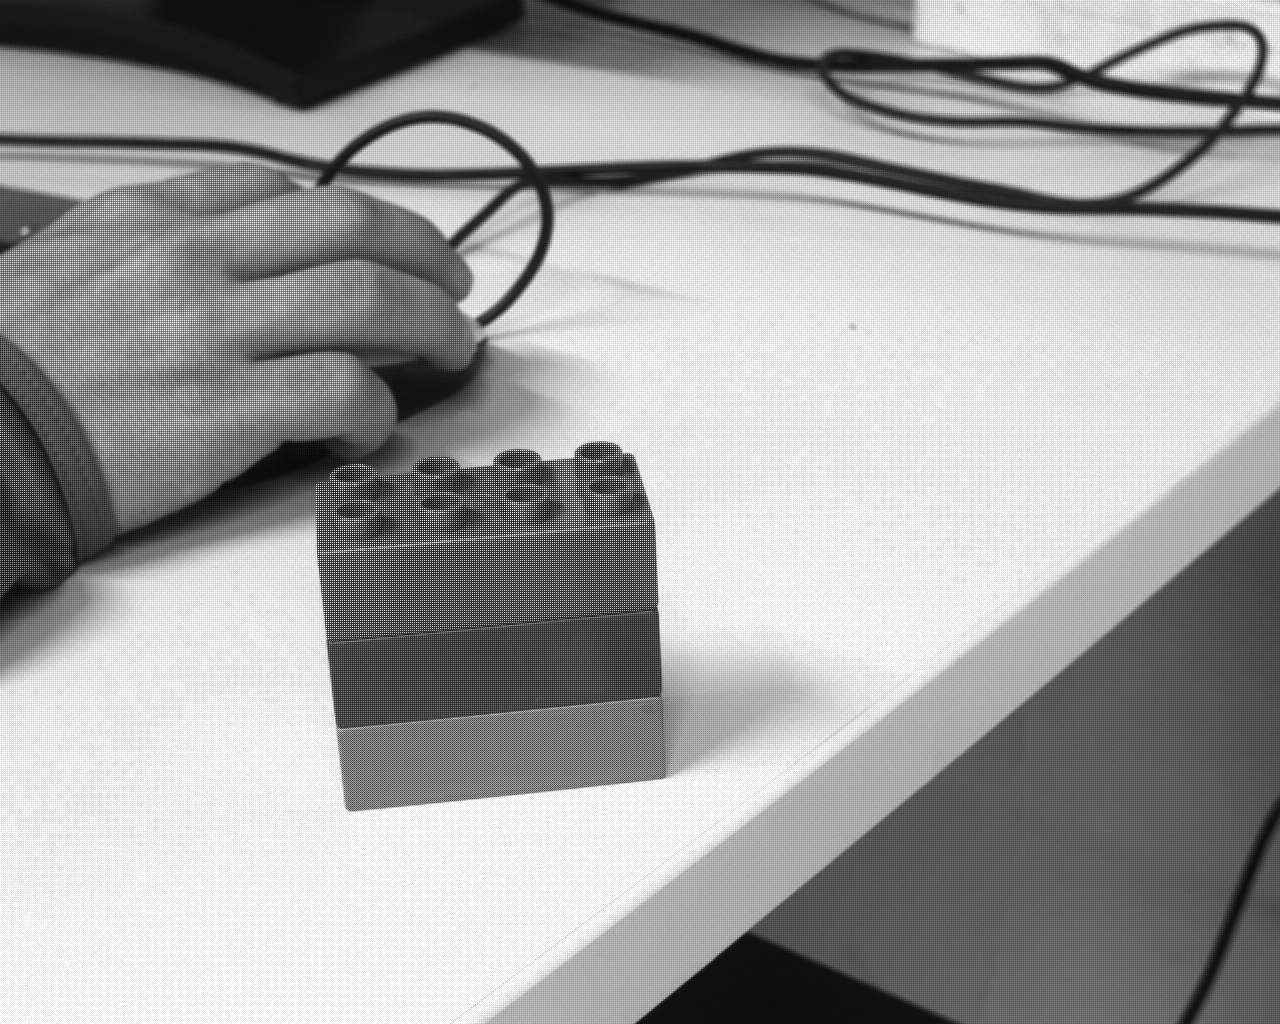
\includegraphics[width=.6\linewidth]{./Bildg_Messtechnik_Lab/ColorImageAcquisition/pictures/bayer1.png}
%% \caption{Raw Image from camera, showing Bayer pattern}
%% \label{fig:imgAcq_Raw}
%%\end{figure}

\begin{figure}[ht]
\centering
\begin{tikzpicture}[zoomboxarray,
    zoomboxarray columns=1,
    zoomboxarray rows=1,
    connect zoomboxes,
    zoombox paths/.append style={ultra thick, red}]
    \node [image node] { 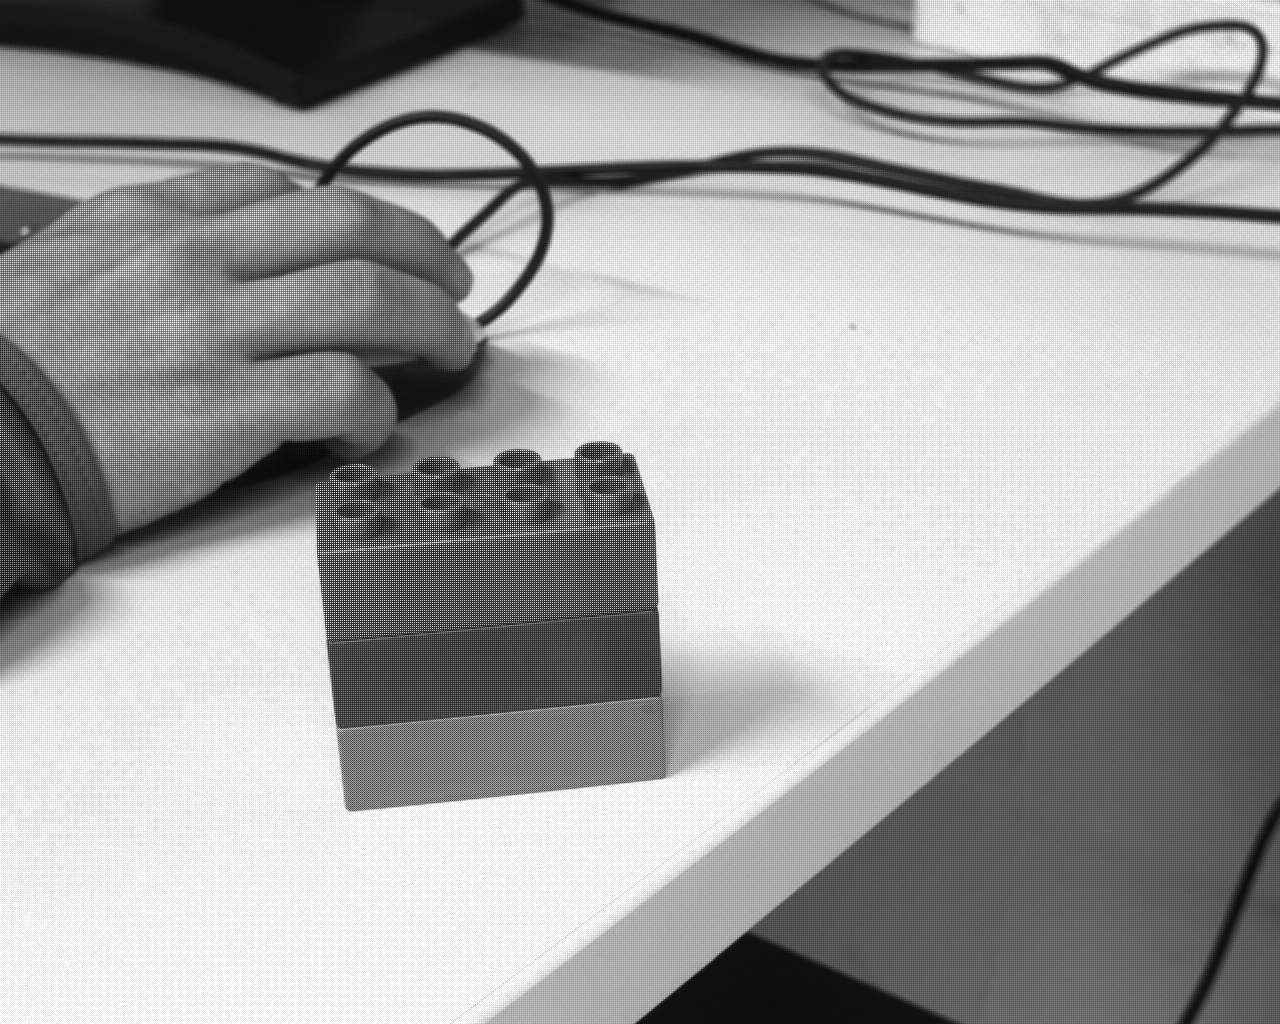
\includegraphics[width=0.45\textwidth]{./Bildg_Messtechnik_Lab/ColorImageAcquisition/pictures/bayer1.png} };
    \zoombox[magnification=10]{0.36,0.38}
\end{tikzpicture}
\caption{Raw image from camera, showing Bayer pattern. The Lego bricks are red, blue and green respectively}\label{fig:imgAcq_Raw}
\end{figure}

This image is fed into the MATLAB script shown in \cref{lst:imgAcq_Raw1}. The user is prompted to select image regions representing red, green and blue areas respectively. The best-fitting cells in an $8 \times 8$ pixels grid are then displayed.

\begin{lstlisting}[float,floatplacement=h!,label=lst:imgAcq_Raw1, caption=Matlab script to show bayer pattern of acquired image]
raw = imread('pictures/bayer1.png');

[h, w] = size(raw);

%select 3 points with given color
figure;
[c, r, ~] = impixel(raw); close;

c = round(c/8) * 8 +1; %choose nearest cell in 8x8 grid
r = round(r/8) * 8 +1; %choose nearest cell in 8x8 grid

im_red   = raw(r(1)-4:r(1)+3, c(1)-4:c(1)+3);
im_green = raw(r(2)-4:r(2)+3, c(2)-4:c(2)+3);
im_blue  = raw(r(3)-4:r(3)+3, c(3)-4:c(3)+3);

figure; %display red, green and blue cells
subplot(2,2,1);
imshow(im_red);
title('Red');

subplot(2,2,2);
imshow(im_green);
title('Green');

subplot(2,2,3);
imshow(im_blue);
title('Blue');
\end{lstlisting}

The result, shown in \cref{fig:imgAcq_BayerRGB}, indicates a $4 \times 4$ bayer pattern with filters for red on the top-left pixel, green on both top-right and bottom-left pixels and blue on the bottom-right pixel.

\begin{figure}[ht!]
 \centering
 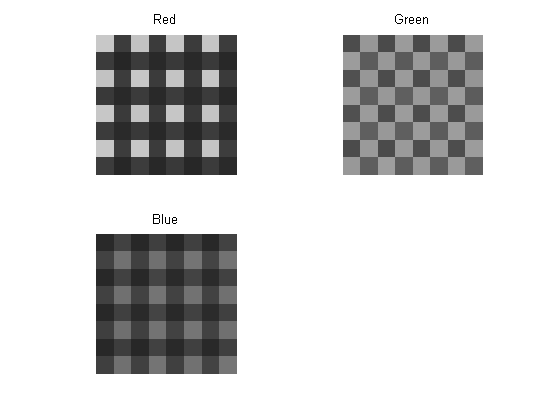
\includegraphics[trim=60px 40px 60px 0, clip, width=.6\textwidth]{./Bildg_Messtechnik_Lab/ColorImageAcquisition/html/main_01.png}
 \caption{Extracted bayer patterns from raw image}
 \label{fig:imgAcq_BayerRGB}
\end{figure}

\clearpage
Using this information, it is possible to write code to convert the raw image to a full rgb picture. A very simple implementation is shown in \cref{lst:imgAcq_Raw2}. Using this script on the initial image results in the image shown in \cref{fig:imgAcq_Interp}.


\begin{lstlisting}[label=lst:imgAcq_Raw2, caption=Matlab script to convert raw pictures to RGB]
img2 = zeros(h,w,3);

x = 1:w;
y = 1:h;
rawD = double(raw);
img2(:,:,1) = interp2(1:2:w,1:2:h,rawD(1:2:end,1:2:end), x', y);
img2(:,:,2) = interp2(1:2:w,1:2:h,rawD(1:2:end,2:2:end) + pat_green(2:2:end,1:2:end), x', y);
img2(:,:,3) = interp2(1:2:w,1:2:h,rawD(2:2:end,2:2:end), x', y);

figure;
imshow(uint8(img2));
\end{lstlisting}

\begin{figure}[t]
 \centering
 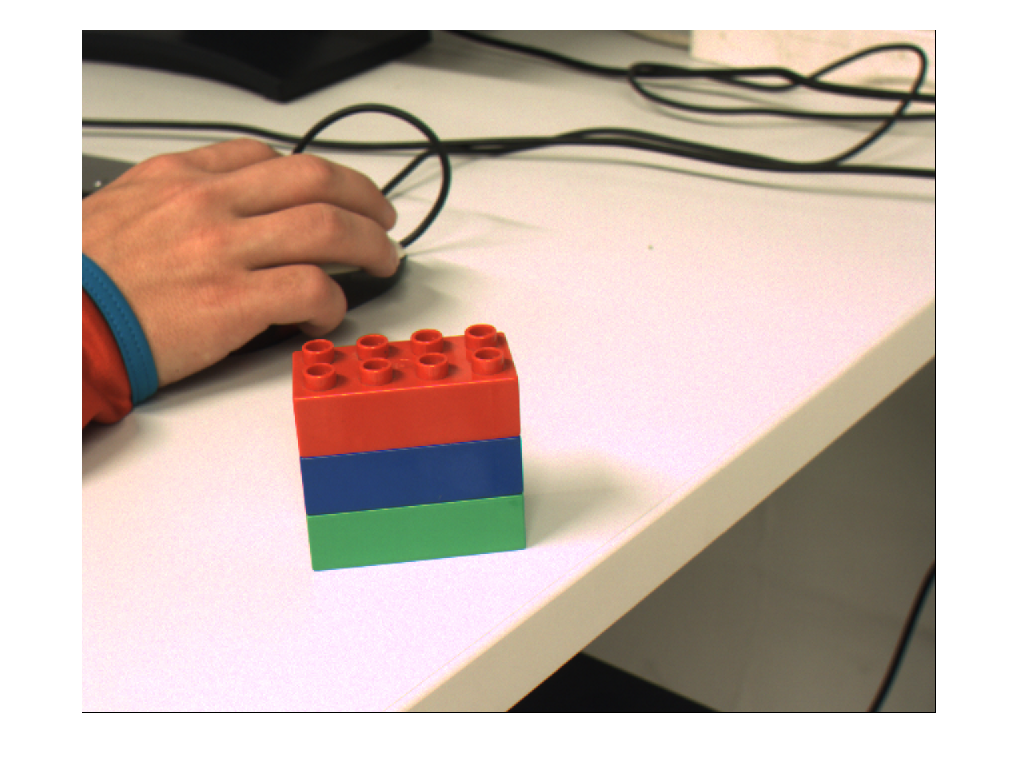
\includegraphics[width=.6\textwidth]{./Bildg_Messtechnik_Lab/ColorImageAcquisition/html/main_02.png}
 \caption{Interpolated RGB image from raw image in \cref{fig:imgAcq_Raw}}  \label{fig:imgAcq_Interp}
\end{figure}

\subsection{Discussion}
Looking at line 7 of \cref{lst:imgAcq_Raw2} and \cref{fig:imgAcq_BayerRGB} shows that the green pixels are only half as bright as the red and blue pixels, but there are twice as many on the whole sensor.

This is the so-called ``bayer pattern''. Green pixels dominate, because green is the dominant color for brightness (and therefore contrast) in the human vision spectrum.


\clearpage
\section{Color Spaces} \label{sec:colSpa}

\subsection{Problem statement}

Using a color camera perform the following tasks:

\begin{itemize}
 \item Capture color images of a scene comprising different colored objects under changing illumination conditions $(N \geq 3)$
 \item Tansform the obtained images into the following color spaces:
 \begin{itemize}
  \item RGB 
  \item HSV
  \item Lab 
  \item XYZ
 \end{itemize}
 \item Discuss how the changing illumination effects the channels of the particular color spaces. What are the possible applications of the individual color spaces?
\end{itemize}

\subsection{Solution}

A nicely colored scene was created and images under different illumination conditions were taken. These images are shown in \cref{fig:colSpa1}.

\begin{figure}[ht!]
\centering
\begin{subfigure}{.3\textwidth}
  \centering
  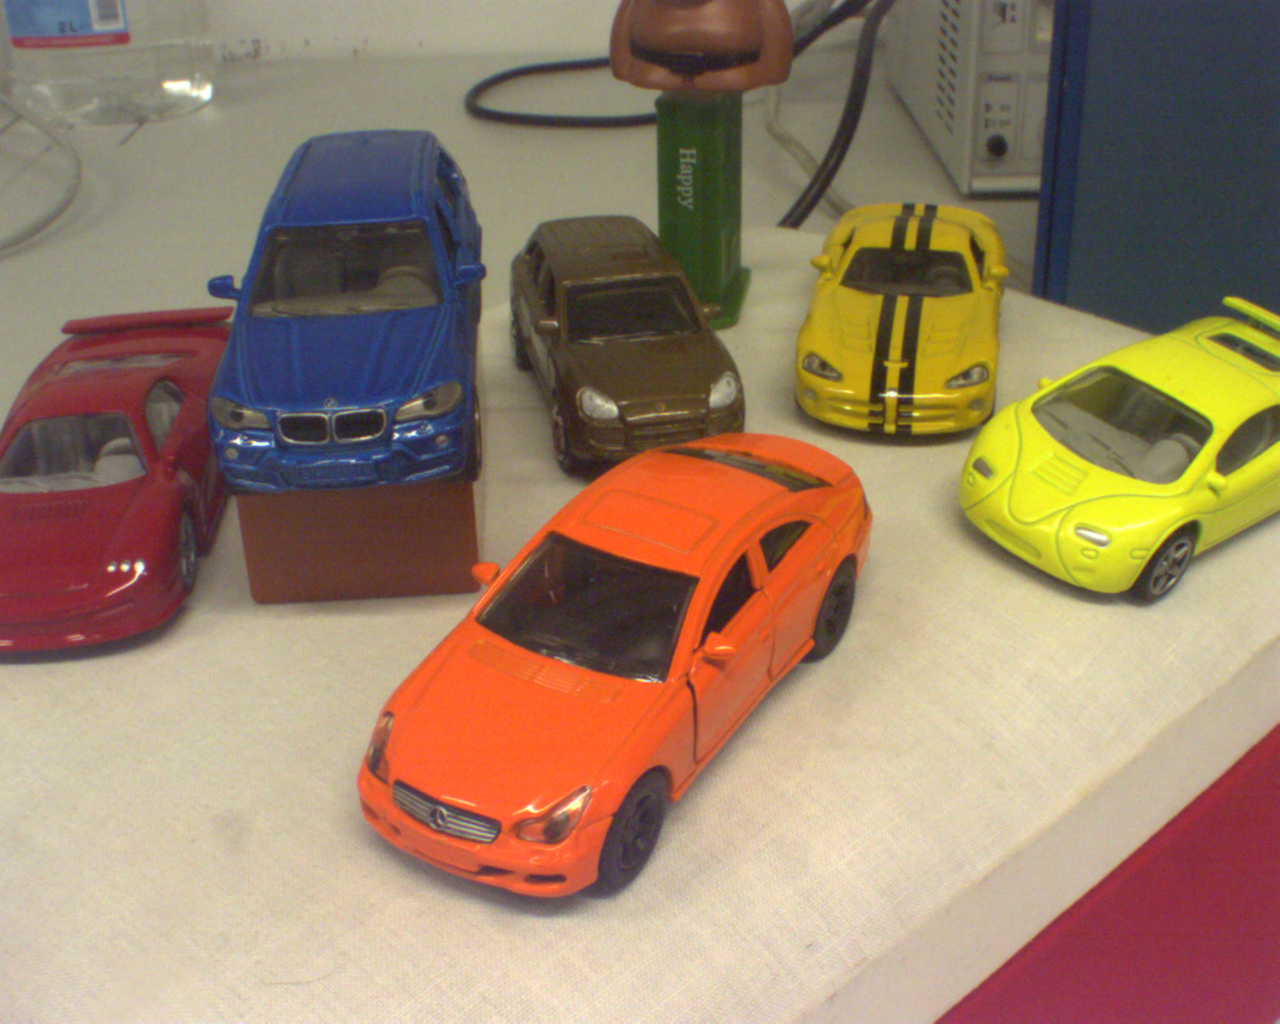
\includegraphics[width=.8\linewidth]{./Bildg_Messtechnik_Lab/ColorSpaces/pictures/bild_ohne.png}
  \caption{room lights}
\end{subfigure}
\begin{subfigure}{.3\textwidth}
  \centering
  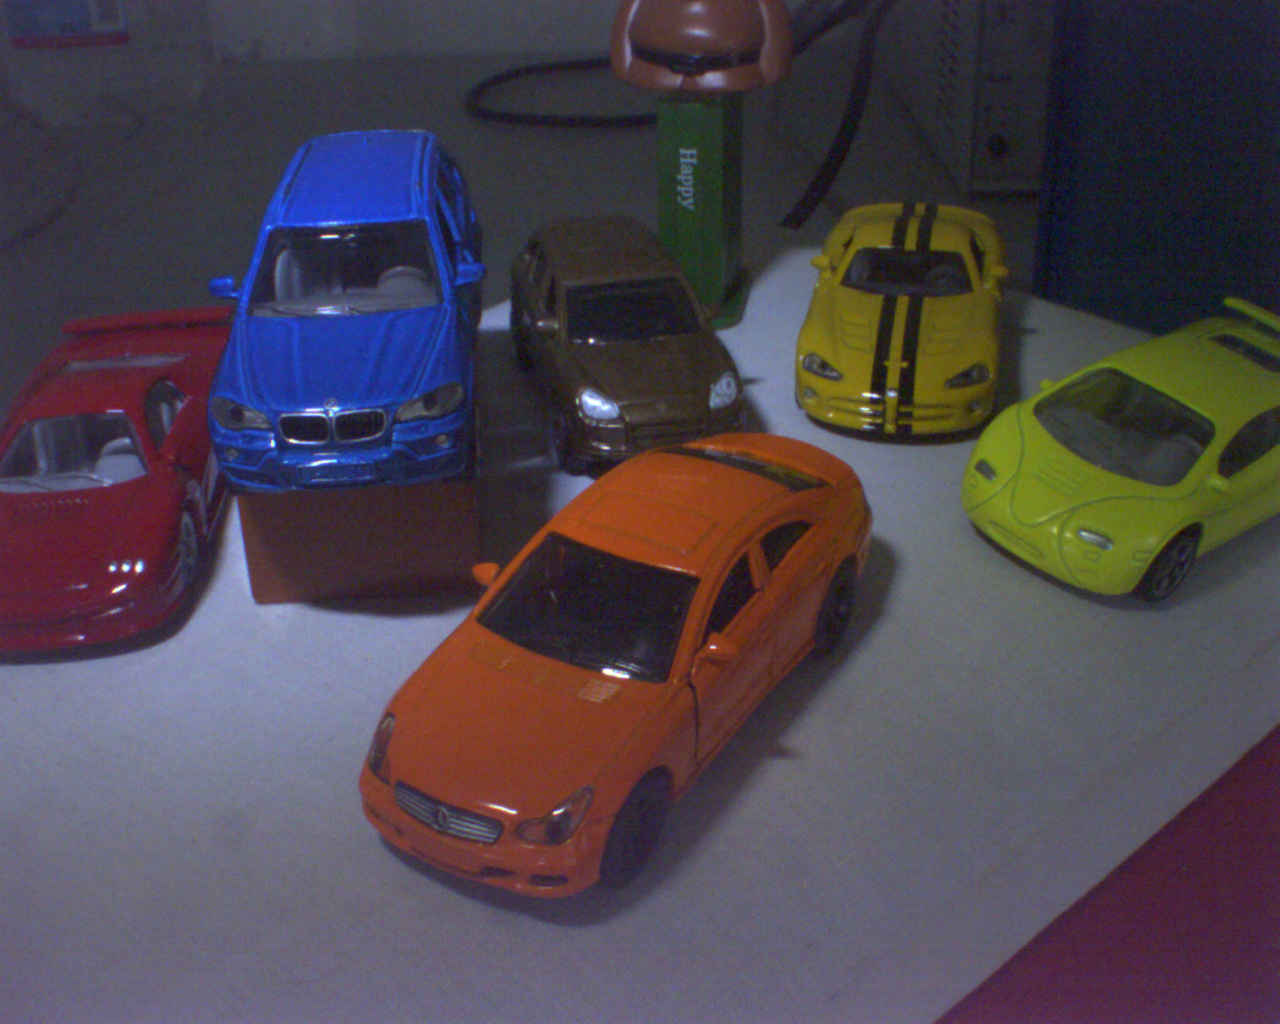
\includegraphics[width=.8\linewidth]{./Bildg_Messtechnik_Lab/ColorSpaces/pictures/bild_led.png}
  \caption{led lamp}
\end{subfigure}
\begin{subfigure}{.3\textwidth}
  \centering
  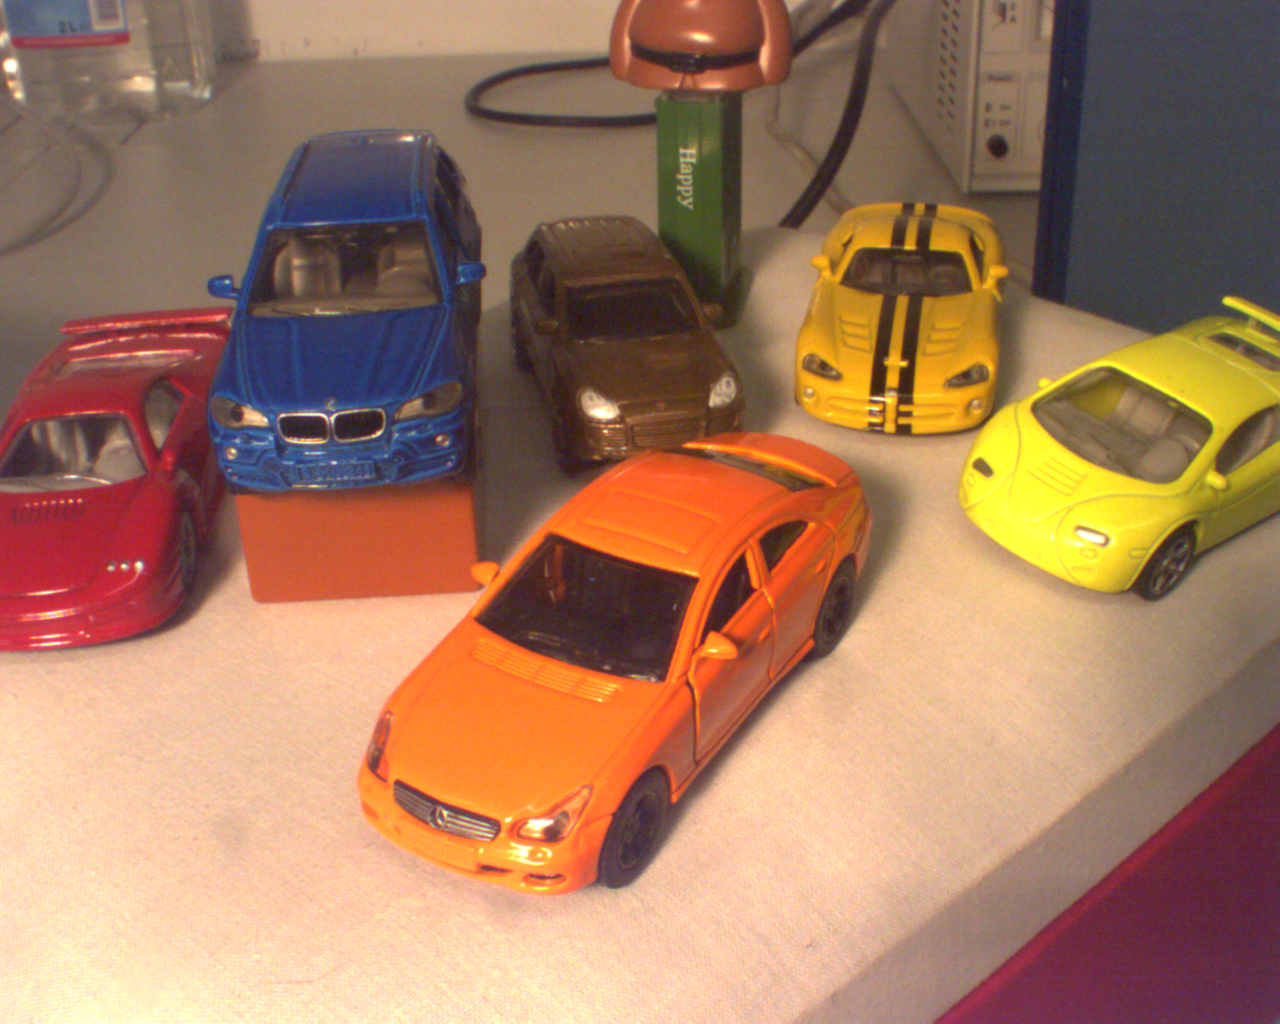
\includegraphics[width=.8\linewidth]{./Bildg_Messtechnik_Lab/ColorSpaces/pictures/bild_strahler.png}
  \caption{halogen lamp}
\end{subfigure}
\caption{Same scene under different illumination conditions}
\label{fig:colSpa1}
\end{figure}

These images were then transformed into HSV, Lab and XYZ color spaces using a MATLAB script. \lstinline{rgb2hsv(..)} is implemented by MATLAB, transformation into the other color spaces was implemented like in \cref{lst:colSpa_Help}.

\begin{lstlisting}[label=lst:colSpa_Help, caption=Helper functions to convert from RGB to Lab and XYZ]
function imgLab = rgb2lab(img)
    C = makecform('srgb2lab');
    imgLab = applycform(img, C);
end

function imgXyz = rgb2xyz(img)
    C = makecform('srgb2xyz');
    imgXyz = applycform(img, C);
end
\end{lstlisting}

\newpage
\begin{figure}[ht!]
\centering
\begin{subfigure}{\textwidth}
  \centering
  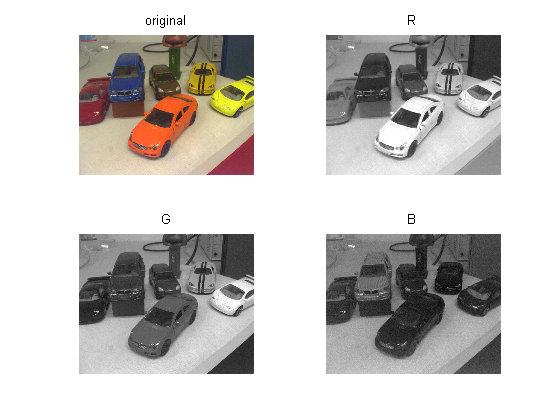
\includegraphics[trim=60px 40px 60px 0, clip, height=7.3cm]{./Bildg_Messtechnik_Lab/ColorSpaces/html/main_01.png}
  \caption{room lights}
\end{subfigure}
\begin{subfigure}{\textwidth}
  \centering
  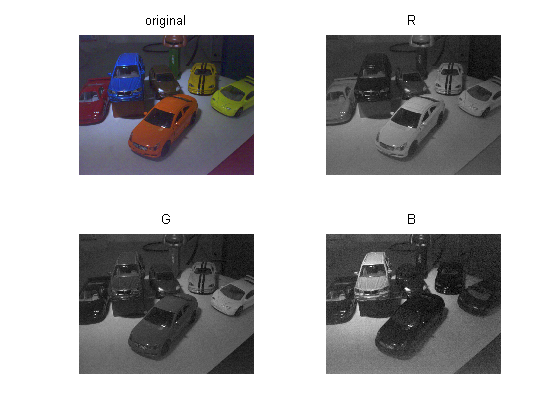
\includegraphics[trim=60px 40px 60px 0, clip, height=7.3cm]{./Bildg_Messtechnik_Lab/ColorSpaces/html/main_05.png}
  \caption{led lamp}
\end{subfigure}
\begin{subfigure}{\textwidth}
  \centering
  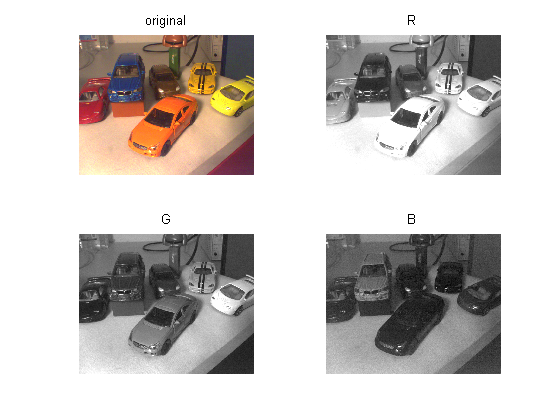
\includegraphics[trim=60px 40px 60px 0, clip, height=7.3cm]{./Bildg_Messtechnik_Lab/ColorSpaces/html/main_09.png}
  \caption{halogen lamp}
\end{subfigure}
\caption{RGB channels of the same scene under different illumination conditions}
\label{fig:colSpa_RGB}
\end{figure}

\newpage
\begin{figure}[ht!]
\centering
\begin{subfigure}{\textwidth}
  \centering
  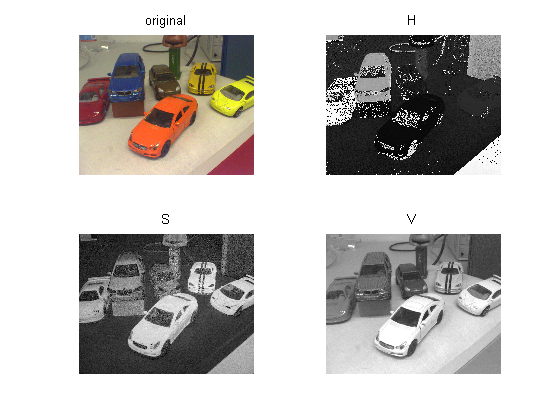
\includegraphics[trim=60px 40px 60px 0, clip, height=7.3cm]{./Bildg_Messtechnik_Lab/ColorSpaces/html/main_02.png}
  \caption{room lights}
\end{subfigure}
\begin{subfigure}{\textwidth}
  \centering
  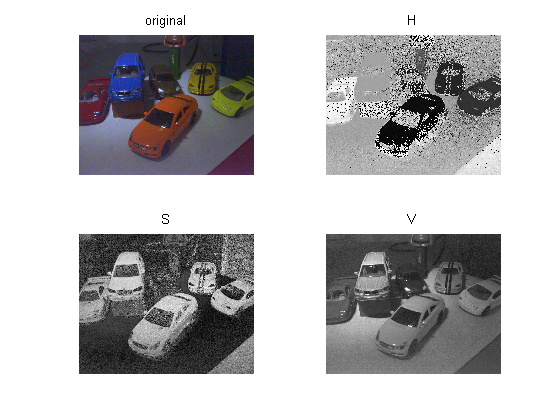
\includegraphics[trim=60px 40px 60px 0, clip, height=7.3cm]{./Bildg_Messtechnik_Lab/ColorSpaces/html/main_06.png}
  \caption{led lamp} \label{fig:colSpa_HSVb}
\end{subfigure}
\begin{subfigure}{\textwidth}
  \centering
  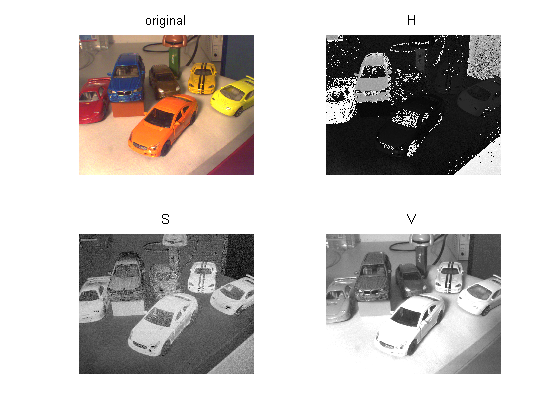
\includegraphics[trim=60px 40px 60px 0, clip, height=7.3cm]{./Bildg_Messtechnik_Lab/ColorSpaces/html/main_10.png}
  \caption{halogen lamp}
\end{subfigure}
\caption{HSV channels of the same scene under different illumination conditions}
\label{fig:colSpa_HSV}
\end{figure}

\newpage
\begin{figure}[ht!]
\centering
\begin{subfigure}{\textwidth}
  \centering
  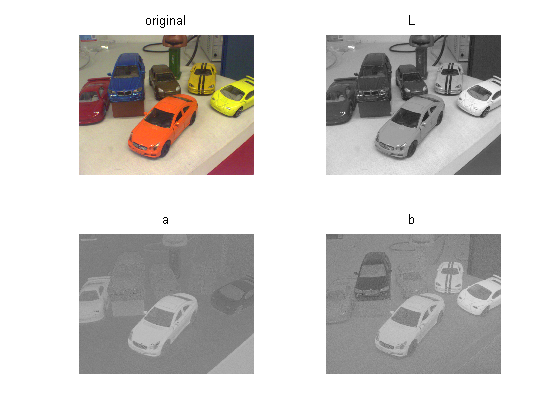
\includegraphics[trim=60px 40px 60px 0, clip, height=7.3cm]{./Bildg_Messtechnik_Lab/ColorSpaces/html/main_03.png}
  \caption{room lights}
\end{subfigure}
\begin{subfigure}{\textwidth}
  \centering
  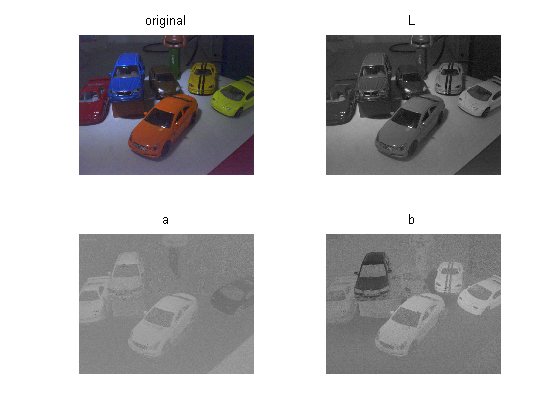
\includegraphics[trim=60px 40px 60px 0, clip, height=7.3cm]{./Bildg_Messtechnik_Lab/ColorSpaces/html/main_07.png}
  \caption{led lamp}
\end{subfigure}
\begin{subfigure}{\textwidth}
  \centering
  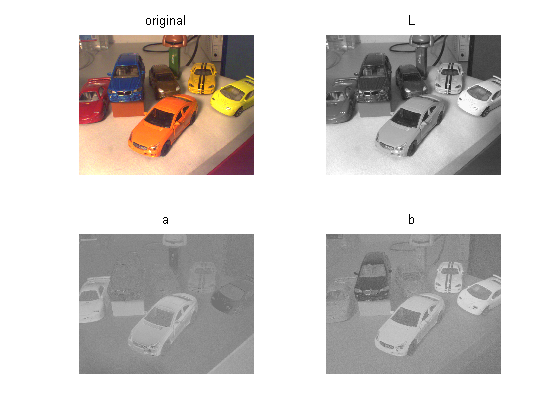
\includegraphics[trim=60px 40px 60px 0, clip, height=7.3cm]{./Bildg_Messtechnik_Lab/ColorSpaces/html/main_11.png}
  \caption{halogen lamp}
\end{subfigure}
\caption{Lab channels of the same scene under different illumination conditions}
\label{fig:colSpa_Lab}
\end{figure}

\newpage
\begin{figure}[ht!]
\centering
\begin{subfigure}{\textwidth}
  \centering
  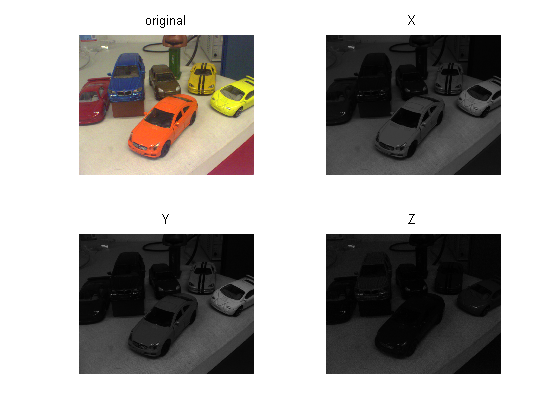
\includegraphics[trim=60px 40px 60px 0, clip, height=7.3cm]{./Bildg_Messtechnik_Lab/ColorSpaces/html/main_04.png}
  \caption{room lights}
\end{subfigure}
\begin{subfigure}{\textwidth}
  \centering
  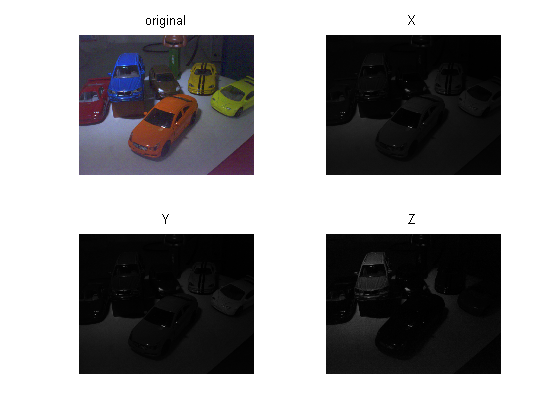
\includegraphics[trim=60px 40px 60px 0, clip, height=7.3cm]{./Bildg_Messtechnik_Lab/ColorSpaces/html/main_08.png}
  \caption{led lamp}
\end{subfigure}
\begin{subfigure}{\textwidth}
  \centering
  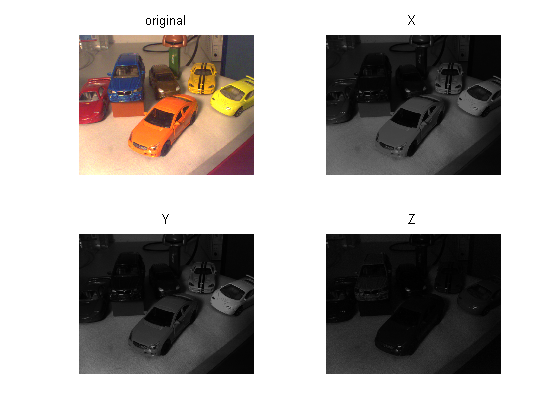
\includegraphics[trim=60px 40px 60px 0, clip, height=7.3cm]{./Bildg_Messtechnik_Lab/ColorSpaces/html/main_12.png}
  \caption{halogen lamp}
\end{subfigure}
\caption{XYZ channels of the same scene under different illumination conditions}
\label{fig:colSpa_XYZ}
\end{figure}

\clearpage
\subsection{Discussion}
Comparing the three images in different color spaces shows some interesting features:
\begin{itemize}
 \item \textbf{RGB}: All channels vary much with different illumination conditions, consequently this color space is not very practical for filtering out color information. It is, however, the usual internal representation of digital images.
 \item \textbf{HSV}: Separating \textbf Hue, \textbf Saturation and \textbf Value is useful for several tasks in image processing. In this case H and S channels are relatively independent from illumination strength.\\
 The Hue-Channel-Image for \cref{fig:colSpa_HSVb} looks quite different. However, since Hue is periodic, dark ($0.0$) and bright ($1.0$) represent the same color (red).
 \item \textbf{Lab}: The Lab color space splits representation in \textbf Lightness and \textbf{a},\textbf{b} for color opponent dimensions. It is designed to mimic human color perception and therefore yields a,b-channel values that are relatively independent of illumination. Just like human vision can identify colors under almost any illumination condition.
 \item \textbf{XYZ}: The XYZ color space was also designed with human perception in mind. The X,Y and Z-channels directly represent the light intensities in the human perception spectrum where X is red, Y is green, and Z is blue.
\end{itemize}

\newpage
\FloatBarrier
\section{Color Constancy}

\subsection{Problem statement}

Using a color camera perform the following tasts:
\begin{itemize}
 \item Capture color images of a scene under different illumination conditions.
 \item Implement different algorithms to perform a white balance on your images:
 \begin{itemize}
  \item White patch retinex algorithm.
  \item White patch retinex algorithm using histogram information
  \item Gray world assumption
 \end{itemize}
 \item Discuss your results.
\end{itemize}

\subsection{Solution}
The images from \cref{sec:colSpa} were used for this exercise. The three different algorithms from appendix A in the laboratory handout\cite{HO} were implemented in MATLAB. The implementation is shown in \cref{lst:colConst_WPR,lst:colConst_WPRH,lst:colConst_GW}.


\subsection{Discussion}
The results shown in \cref{fig:colConst} show the poor performance of any of the white balance algorithms. \textit{whitePatchRetinex} always maxes each color out, so it doesn't change anything in the image.
\textit{whitePatchRetinexHist} performs significantly better in terms of brightness compensation, however color remains unchanged. \textit{grayWorld} performs exactly like \textit{whitePatchRetinexHist}.\\[2em]

\begin{lstlisting}[label=lst:colConst_WPR, caption=MATLAB implementation of whitePatchRetinex]
function [ img_out ] = whitePatchRetinex( img_in )

img_out = double(img_in);

L_i_max(1) = max(max(img_in(:,:,1)));
L_i_max(2) = max(max(img_in(:,:,2)));
L_i_max(3) = max(max(img_in(:,:,3)));

L_i_max %well... this is more often than not [255 255 255]

for i=1:3
    img_out(:,:,i) = img_out(:,:,i) ./ double(L_i_max(i)) .* 255;
end

img_out = uint8(img_out);
end
\end{lstlisting}
\newpage


\begin{lstlisting}[label=lst:colConst_WPRH, caption=MATLAB implementation of whitePatchRetinexHist]
function [ img_out ] = whitePatchRetinexHist( img_in )

img_out = double(img_in);

img_r = img_in(:,:,1);
img_r = sort(img_r(:), 'descend');
L_i_max(1) = img_r(floor(numel(img_r)*0.05));

img_g = img_in(:,:,1);
img_g = sort(img_g(:), 'descend');
L_i_max(2) = img_g(floor(numel(img_g)*0.05));

img_b = img_in(:,:,1);
img_b = sort(img_b(:), 'descend');
L_i_max(3) = img_b(floor(numel(img_b)*0.05));

for i=1:3
    img_out(:,:,i) = img_out(:,:,i) ./ double(L_i_max(i)) .* 255;
end

img_out = uint8(img_out);
end
\end{lstlisting}



\begin{lstlisting}[label=lst:colConst_GW, caption=MATLAB implementation of grayWorld]
function [ img_out ] = grayWorld( img_in )

img_out = double(img_in);

img_r = img_in(:,:,1);
L_i_mean(1) = mean(img_r(:));

img_g = img_in(:,:,1);
L_i_mean(2) = mean(img_g(:));

img_b = img_in(:,:,1);
L_i_mean(3) = mean(img_b(:));

for i=1:3
    img_out(:,:,i) = img_out(:,:,i) ./ double(L_i_mean(i));
end

img_out_v = sort(img_out(:),'descend');
max_out = img_out_v(floor(numel(img_out)*0.10));

img_out = img_out / max_out * 255;
img_out = min(img_out, 255); %clip values over 255

img_out = uint8(img_out);
end
\end{lstlisting}



\newpage
\begin{figure}[ht!]
\centering
\begin{subfigure}{\textwidth}
  \centering
  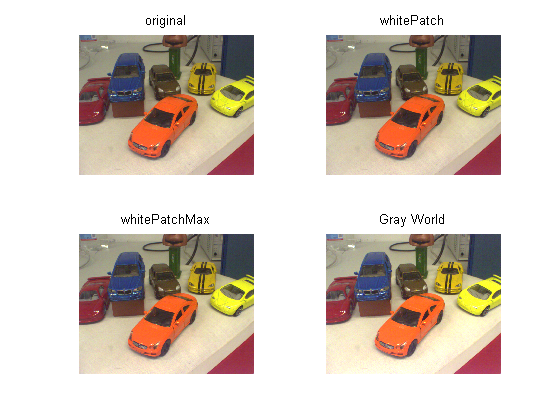
\includegraphics[trim=40px 40px 40px 0, clip, height=7.3cm]{./Bildg_Messtechnik_Lab/ColorConstancy/html/main_01.png}
  \caption{room lights}
\end{subfigure}
\begin{subfigure}{\textwidth}
  \centering
  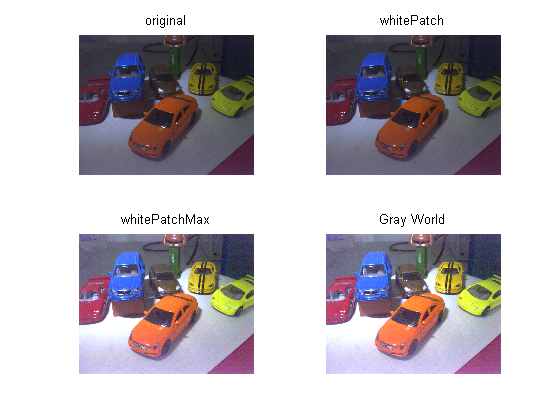
\includegraphics[trim=40px 40px 40px 0, clip, height=7.3cm]{./Bildg_Messtechnik_Lab/ColorConstancy/html/main_03.png}
  \caption{led lamp}
\end{subfigure}
\begin{subfigure}{\textwidth}
  \centering
  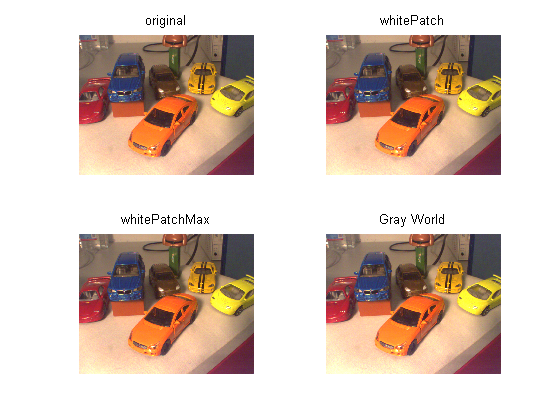
\includegraphics[trim=40px 40px 40px 0, clip, height=7.3cm]{./Bildg_Messtechnik_Lab/ColorConstancy/html/main_02.png}
  \caption{halogen lamp}
\end{subfigure}
\caption{Comparison of different white balance algorithms}
\label{fig:colConst}
\end{figure}
\FloatBarrier


\section{Color Calibration}

\subsection{Problem statement}

Using a color camera perform the following tasts:

\begin{itemize}
 \item Capture a color image of a color reference target under uniform illumination conditions.
 \item Perform a radiometric calibration of your camera. To do so find a mapping $\bm{M} \in R^{3 \times 3}$ that transforms the image pixel color value $\bm{c}(x,y) = (c_r(x,y), c_g(x,y), c_b(x,y))^T$ of a color target patch into the known reference value $\bm{r}(x,y) = (r_r(x,y), r_g(x,y), r_b(x,y))^T$.
 \item Compare the color differences to the ground truth values before and after the calibration of the camera.
 \item Discuss your results.
\end{itemize}

\subsection{Solution}

\begin{figure}[ht!]
\centering
\begin{subfigure}{0.49\textwidth}
  \centering
  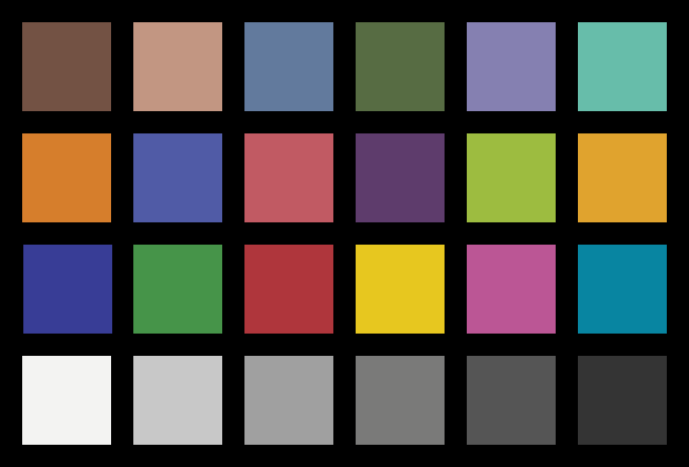
\includegraphics[height=5cm]{./Bildg_Messtechnik_Lab/ColorCalibration/color_checker.png}
  \caption{reference target}
\end{subfigure}%
\begin{subfigure}{0.49\textwidth}
  \centering
  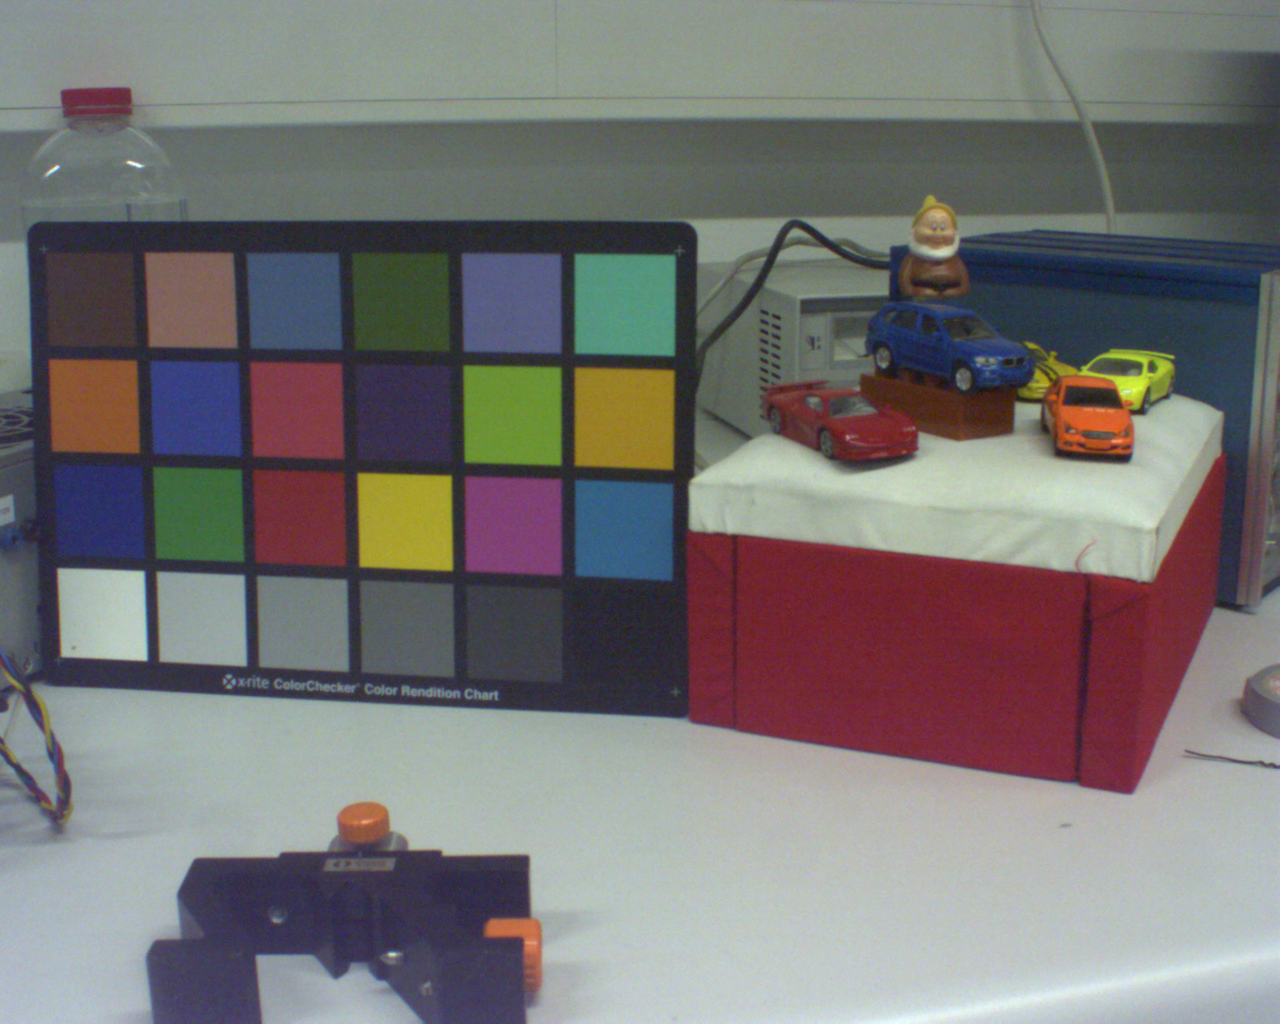
\includegraphics[clip, trim=0 4cm 0 4cm, width=\textwidth]{./Bildg_Messtechnik_Lab/ColorCalibration/pictures/pic_D50.png}
  \caption{picture of target}
\end{subfigure}
\caption{Color reference target and picture}
\label{fig:colCal_ref}
\end{figure}

\newcommand{\R}{\mathbb{R}}

A picture of the printed reference target was taken and loaded in a Matlab-script. Based on the color information of this picture and the reference colors two strategies to color-calibrate the camera were implemented. \\

The first uses a corespondence-matrix $M \in \R ^{3\times 3}$, such that
\begin{align*}  r = M c \text{,} \end{align*}
where $c \in \R^3$ is the pixel color of the image and $r \in \R^3$ is the corrected color.

For this, four color corespondences where manually chosen on the picture and $M$ fitted accordingly using the algorithm shown in \cref{lst:colCal_calibCam}. \Cref{fig:colCal_pict1} shows the adjusted picture.

Since this calibration method only allows for linear adjustments, it fails miserably when trying to calibrate badly distorted colors (like the light blue square in the third row). \\

The second approach fits the color channels over a few gray squares and thus allows non-linear corrections. This strategy was already implemented in \textit{grayValueCurveFitting} and only used by us. \Cref{fig:colCal_pict2,fig:colCal_pict3} shows the fitting functions and the resulting adjusted image.

\begin{lstlisting}[label=lst:colCal_calibCam, caption=MATLAB implementation of calibCam]
function [ n_img ] = calibCam( val_img, val_target, img )
% Color camera calibration
% Input:
%   val_img ... rgb color values of the image (Nx3)
%   val_target ... rgb color values of the calibration pattern (Nx3)
%   img ... original image
%
% Return:
%   n_img ... calibrated image
N = size(val_img,1); % N = number of patches

% mapping M
M = val_img \ val_target;

n_img = img;

% split RGB-image to color channels
imgR = img(:,:,1);
imgG = img(:,:,2);
imgB = img(:,:,3);
img2 = [imgR(:), imgG(:), imgB(:)];

% adjust colors
img2 = M * double(img2)';
img2 = img2';

% reshape color channels back to RGB-image
n_img(:,:,1) = reshape(img2(:,1), size(img,1), size(img,2));
n_img(:,:,2) = reshape(img2(:,2), size(img,1), size(img,2));
n_img(:,:,3) = reshape(img2(:,3), size(img,1), size(img,2));
\end{lstlisting}

\subsection{Discussion}
The colors of the six squares in the third row were compared with the reference colors, the mean difference of each can be found in \cref{tab:colCal_err}. Obviously, while calibrating improves the color-correctness, a small error still remains.

Comparing \cref{fig:colCal_pict1,fig:colCal_pict3} shows that the second, non-linear method, produces more natural images with better white-balance.

\sisetup{table-format=2.1,table-auto-round}
\begin{table}[ht!]
  \centering
  \caption{Mean color difference before and after calibration} \label{tab:colCal_err}
  calculated using $D = \sqrt{\Delta r^2 + \Delta g^2 + \Delta b^2}$ \\
  \begin{tabu}{cSSSSSS}
    \toprule
    Measurement & \multicolumn{6}{c}{Mean color difference on each square} \\
                & {blue} & {green} & {red} & {yelow} & {pink} & {light blue} \\
    \midrule
    uncalibrated image & 69.0302 & 61.9566 & 62.2868 & 79.3880 & 90.9124 & 93.4355 \\
    color calibration  & 13.3420 & 18.6737 & 18.6768 & 34.3115 & 22.4159 & 60.5989 \\
    gray  calibration  & 6.7334 & 30.3153 & 21.1672 & 27.5649 & 18.4197 & 68.7355 \\
    \bottomrule
  \end{tabu} 
\end{table}



\begin{figure}[ht!]
\centering
\begin{subfigure}{0.49\textwidth}
  \centering
  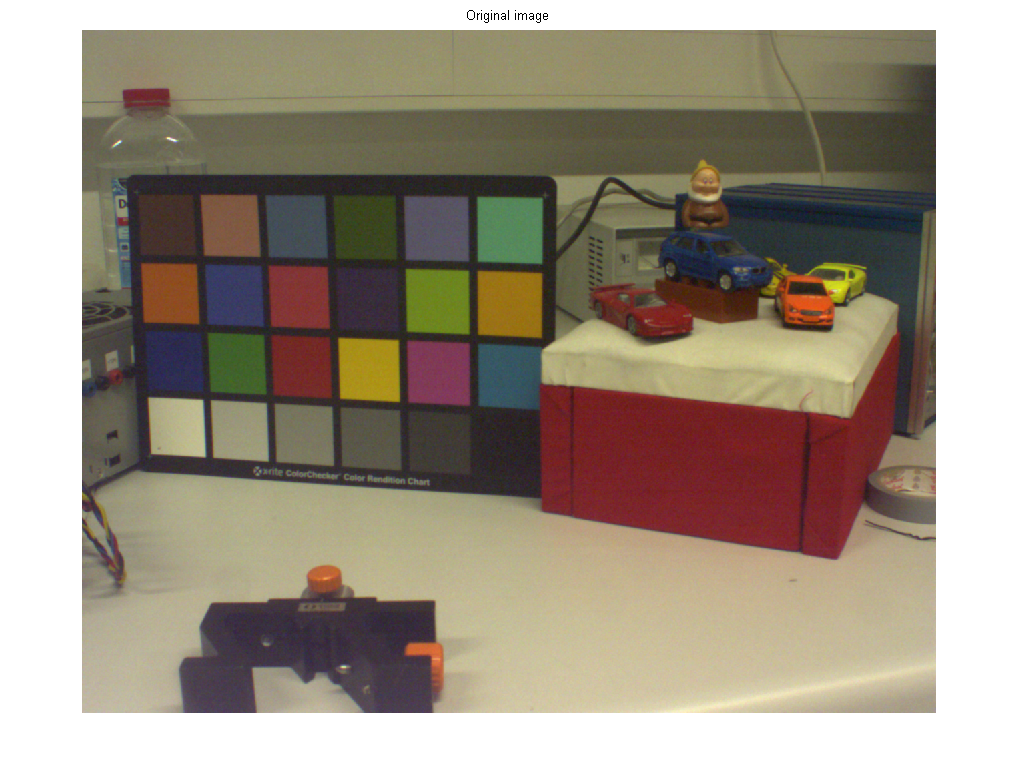
\includegraphics[width=\textwidth]{./Bildg_Messtechnik_Lab/ColorCalibration/html/color_calibration_01.png}
  \caption{uncalibrated image}
\end{subfigure}%
\begin{subfigure}{0.49\textwidth}
  \centering
  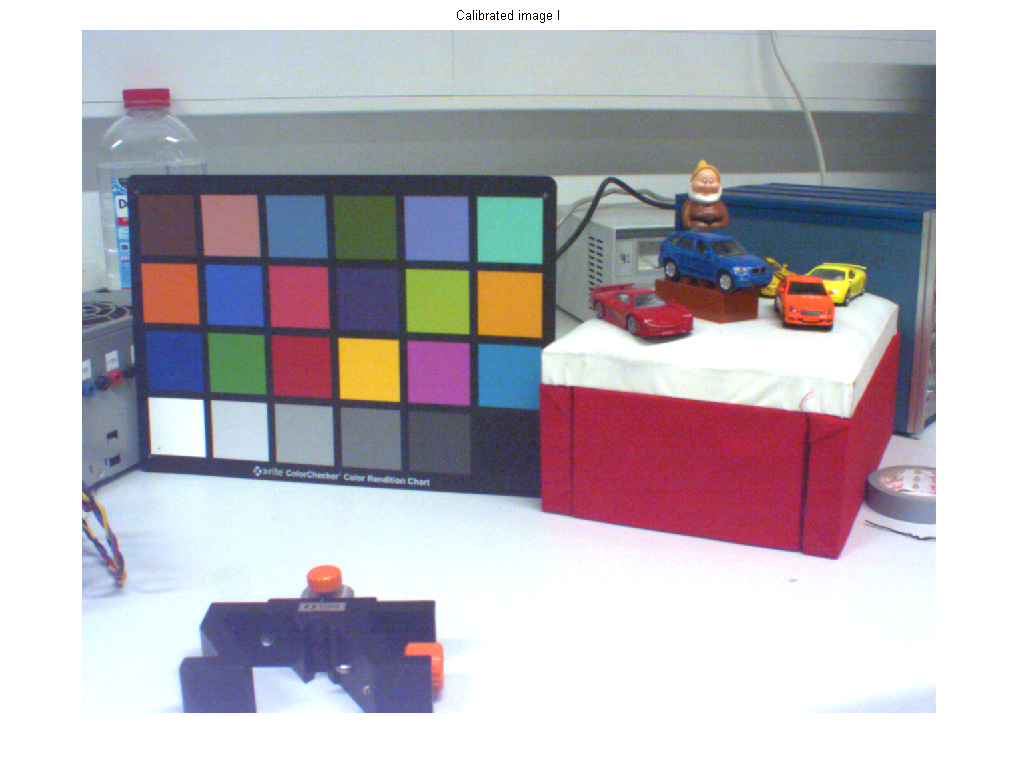
\includegraphics[width=\textwidth]{./Bildg_Messtechnik_Lab/ColorCalibration/html/color_calibration_02.png}
  \caption{color calibration} \label{fig:colCal_pict1}
\end{subfigure}\\
\begin{subfigure}{0.49\textwidth}
  \centering
  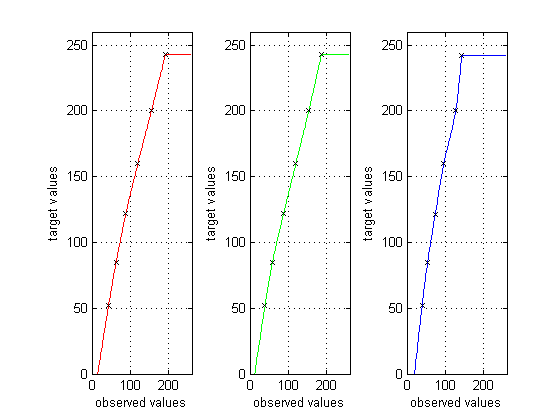
\includegraphics[width=\textwidth]{./Bildg_Messtechnik_Lab/ColorCalibration/html/color_calibration_03.png}
  \caption{color fit for gray calibration} \label{fig:colCal_pict2}
\end{subfigure}%
\begin{subfigure}{0.49\textwidth}
  \centering
  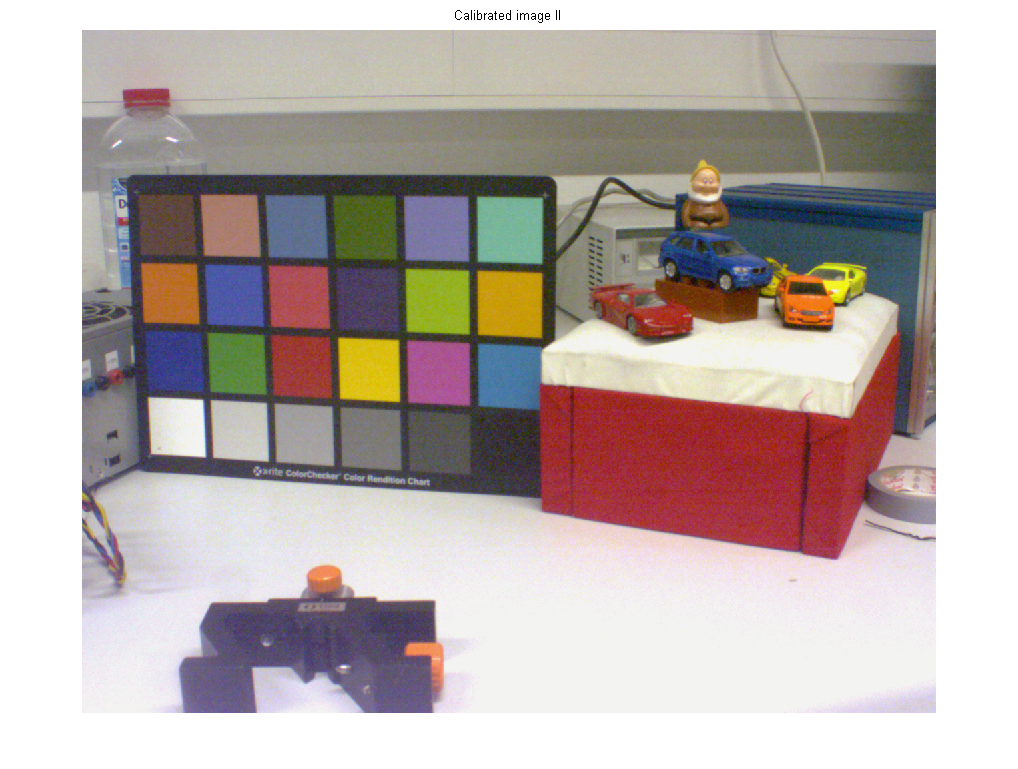
\includegraphics[width=\textwidth]{./Bildg_Messtechnik_Lab/ColorCalibration/html/color_calibration_04.png}
  \caption{gray calibration} \label{fig:colCal_pict3}
\end{subfigure}
\caption{Color calibration results}
\label{fig:colCal_pict}
\end{figure}




%%%
%%% end main document
%%%
%%%%%%%%%%%%%%%%%%%%%%%%%%%%%%%%%%%%%%%%%%%%%%%%%%%%%%%%%%%%%%%%%%%%%%%%%%%%%%%%

% \appendix  %% include it, if something (bibliography, index, ...) follows below

\FloatBarrier
\begin{thebibliography}{XX}
  \bibitem{HO}Laboratory Handout: \textit{Lab2--Color}. \\
    Christoph Feichtenhofer and Thomas Höll, Winter--Term 2016/2017
\end{thebibliography}


%%%%%%%%%%%%%%%%%%%%%%%%%%%%%%%%%%%%%%%%%%%%%%%%%%%%%%%%%%%%%%%%%%%%%%%%%%%%%%%%
%%%
%%% bibliography
%%%
%%% available styles: abbrv, acm, alpha, apalike, ieeetr, plain, siam, unsrt
%%%
% \bibliographystyle{plain}

%%% name of the bibliography file without .bib
%%% e.g.: literatur.bib -> \bibliography{literatur}
% \bibliography{FIXXME}

\end{document}

